\subsection{Storage of fields and index arrays}

How are the fields stored in memory: fastest index etc.

The gauge field ist stored with the local gauge field first with index
{\ttfamily 0 to T*L*L*L-1}, then the right boundary with index
{\ttfamily T*L*L*L to (T+1)*L*L*L-1} and then the left boundary with index
{\ttfamily (T+1)*L*L*L to (T+2)*L*L*L-1}. This means there is no
Even-Odd order in the gauge fields. 

The spinor fields have only size {\ttfamily (VOLUME+RAND)/2}. Thus
there are either only even or only odd sites and the corresponding
boundary stored. There are two index arrays called {\ttfamily lexic2eo}
and {\ttfamily eo2lexic} which map from the whole volume to the even odd
counting and vice versa. {\ttfamily eo2lexic[ix]} returns the lexical
index where {\ttfamily ix} is a even odd index and
{\ttfamily lexic2eo[ix]} returns the even odd index where {\ttfamily ix}
is now a lexical index. {\ttfamily lexic2eosub} maps the lexical index
to the even odd index in a spinor field of half size, thus either with
only odd or with only even points. The latter is a bit dagerous, since
the mapping is not surjective.

With the index array {\ttfamily g\_ipt[t][x][y][z]} one can map the
point $(t,x,y,z)$ to the lexical index. The indices of the next
neighbours of point with lexical index {\ttfamily ix} in positiv and
negative direction $\mu$ you can get with
{\ttfamily g\_iup[ix][$\mu$]} and {\ttfamily g\_idn[ix][$\mu$]}
respectively.

\subsection{Parallelisation}

\begin{figure}[htbp]
\centering
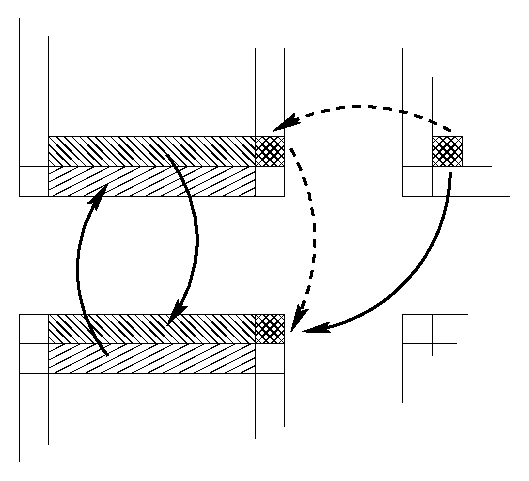
\includegraphics[width=0.65\linewidth]{partition}
\caption{Boundary exchange in a parallel setup. One can see that the
  internal boundary is sended while the external one is received.}
\label{fig:partition}
\end{figure}

The whole lattice can be parallelised in only the $t$-direction (by
defining {\ttfamily PARALLELT} during the compilation) or in $t$-
and $x$-direction (by defining {\ttfamily PARALLELXT}). The exchange is
performed as can be seen schematically in fig.~\ref{fig:partition}.

Note that for the HMC we also need to exchange the edges in order to
make the gauge update correctly.

There are exchange routines available for the gauge fields ({\ttfamily
  xchange\_gauge}), for a (half) spinor field ({\ttfamily
  xchange\_spinor}) and for the derivatives ({\ttfamily xchange\_deri}),
respectively.

In the case of parallelisation in $x$-direction the processors
internal boundary is not continous anymore, but strided. Therefore
{\ttfamily MPI\_Type\_vector} is used in order to avoid to copy the data
in a send buffer before sending it. Not that the external boundary is
still continuous.



%%% Local Variables: 
%%% mode: latex
%%% TeX-master: "main"
%%% End: 
